\graphicspath{{./lab01/Images/}}


\maketitlepage{App Development}{in Android Studio}{Lab 1: Views and events}
\maketocpage

\section{Extensible Markup Language}
Extensible Markup Language (XML) is a markup language, similar to HTML. The main difference being that HTML is designed to display predefined tags while XML is designed to carry arbitrary data. XML documents are structured as trees as can be seen in listing \ref{listing:tree} and are required to have a single root element. A prolog prior to the root element defines the XML version and encoding.
\begin{lstlisting}[style=A_XML, caption={XML tree structure}, label = {listing:tree}]
<?xml version="1.0" encoding="UTF-8"?>
<root_element>
    <element>
        <leaf_element>
        </leaf_element>
    </element>
    <element>
        <element>
            <leaf_element>
            </leaf_element>
        </element>
    </element>
</root_element>
\end{lstlisting}
In Android we use XML to define structure of UI and attributes. Elements can have attributes, which are kept in quotation marks and can describe properties such as id, size and text for elements like buttons and input fields.
\begin{lstlisting}[style=A_XML]
<element attribute1="value1" attribute2="value2"/>
\end{lstlisting}
We also use XML to store information in manifest, UI strings, drawables, styles and layouts. In the program we did in lab 0, we created an activity and with it came a layout XML document. We will take a better look at activities later but for now, we can think of them as a single screen and this layout holds info about its UI components.

\section{Views}
The \href{https://developer.android.com/reference/android/view/View.html}{\texttt{View}} class is the base unit for user interface components. It is responsible for drawing on screen and handling events. It is the root class in the inheritance hierarchy of UI components (disregarding the \texttt{Object} class). Views can be visible component displayed on our screen or invisible containers called \href{https://developer.android.com/reference/android/view/ViewGroup.html}{view groups} to store other visible components. 

\begin{figure}[H]
\centering
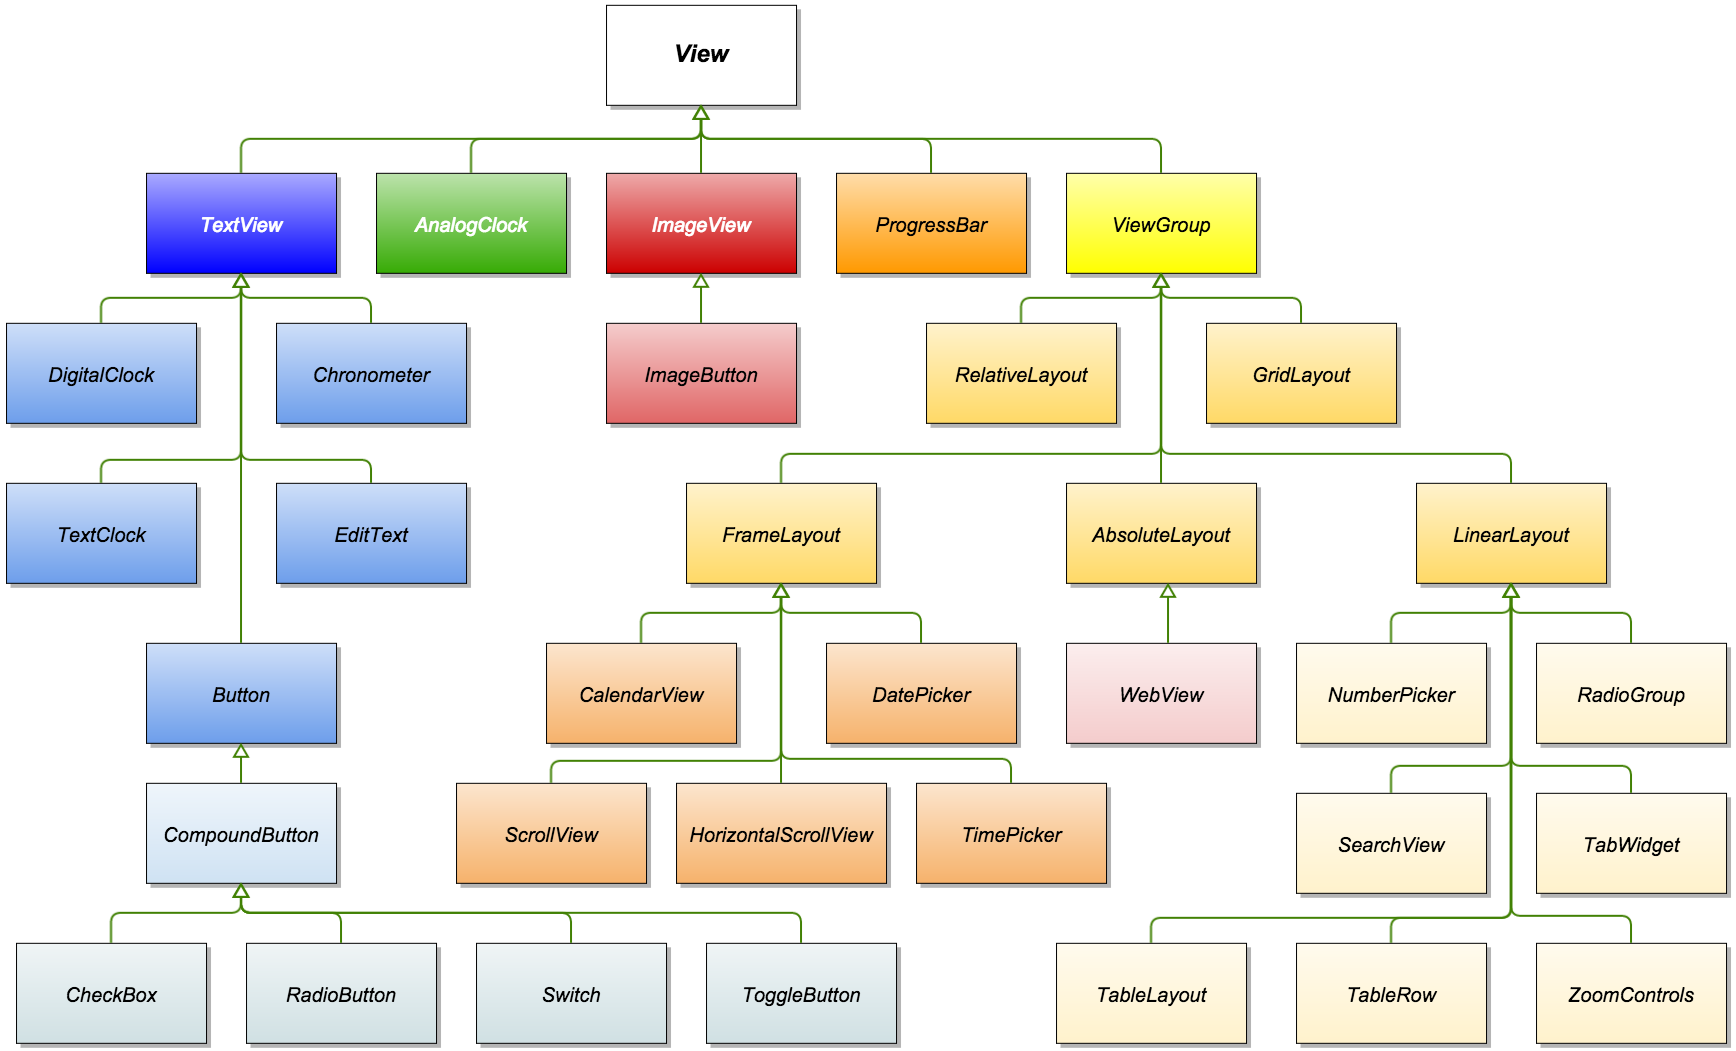
\includegraphics[scale=.375]{ViewHierarchy.png}
\caption{View inheritance hierarchy}
\label{fig:inherhia}
\end{figure}

Our layout XML document will have its own hierarchy of views, formed with an XML tree. The root is some container (view group) and it has some elements which can either be nested containers or drawable UI components. 

\begin{figure}[H]
  \centering
  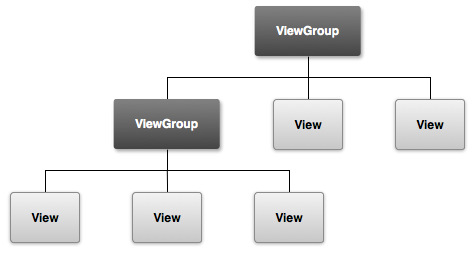
\includegraphics[scale=.5]{viewgroup.png}
  \caption{View hierarchy}
  \label{fig:viewhia}
\end{figure}

\section{Event driven programming}
Unlike the programs we are more used to, there is no main function in Android. It will define what screen (activity) to render when we start the app and from there on, it will react to events, such as swipes and clicks. When such an event occurs, an appropriate event listener is set to handle it. By default, nothing is done but we can implement a method to run if an event occurs.\\

Some events can be implemented in XML. A button is defined and an \texttt{onClick} listener set in listing \ref{listing:xmlhandle}. For this to work, we need to define the method \texttt{public void clickMethod(View view)} in the corresponding activity.
\begin{lstlisting}[style=A_XML, caption={Handling events in XML}, label = {listing:xmlhandle}]
<Button
    android:id="@+id/my_btn"
    android:layout_width="wrap_content"
    android:layout_height="wrap_content"
    android:text="ClickMe" 
    android:onClick="clickMethod"/> <!-- text should be in res/strings -->
\end{lstlisting}
We can also set listeners in Java by finding the view by its id. This is shown using an anonymous class in listing \ref{listing:javahandle} but can also be done with lambdas or classes that implement the \texttt{View.OnClickListener}.
\begin{lstlisting}[style=A_Java, caption={Handling events in Java}, label = {listing:javahandle}]
Button btn = (Button)findViewById(R.id.my_btn);
btn.setOnClickListener(new View.OnClickListener() {
    @Override
    public void onClick(View v) {
        // is called when clicked
    }
});
\end{lstlisting}

\section{Layouts}
Layouts are invisible view groups that allows us to structure our UI. The root element in our layout XML has to be any of the available layouts. There are many layouts available in Android and we will only go over a few.\\

Before we look at the various layouts, we need to address certain XML attributes and units for their values. There are six different units for sizes in Android, seen in table \ref{table:units}, but luckily we will only ever have to use two, sp for fonts and dp for everything else.

\begin{table}[H]
    \centering
    \begin{tabular}{l|l|l}
        Abbreviation & Name & Description \\ 
        \hline
        dp & Density Independent Pixel & 1 pixel in 160 dpi screens (px $=$ dp $\cdot$ (dpi $/ 160$)) \\
        in & Inches & Physical measurement \\
        mm & Millimeters & Physical measurement \\
        pt & Point & Physical measurement \\
        px & Pixel & A single screen pixel \\
        sp & Scale Independent Pixel & Scaled based on user’s font size preference.
    \end{tabular}
    \caption{Size units}
    \label{table:units}
\end{table}%dp, in, mm, pt, px, sp

The attributes to position elements are explained in figures \ref{fig:wah}, \ref{fig:grav} and \ref{fig:pam}.

\begin{figure}[H]
  \centering
  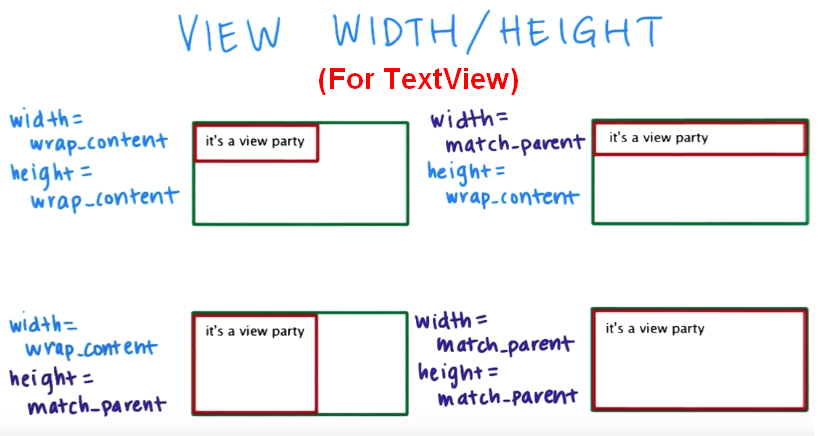
\includegraphics[scale=.35]{width_height.png}
  \caption{Width and height}
  \label{fig:wah}
\end{figure}
\begin{figure}[H]
  \centering
  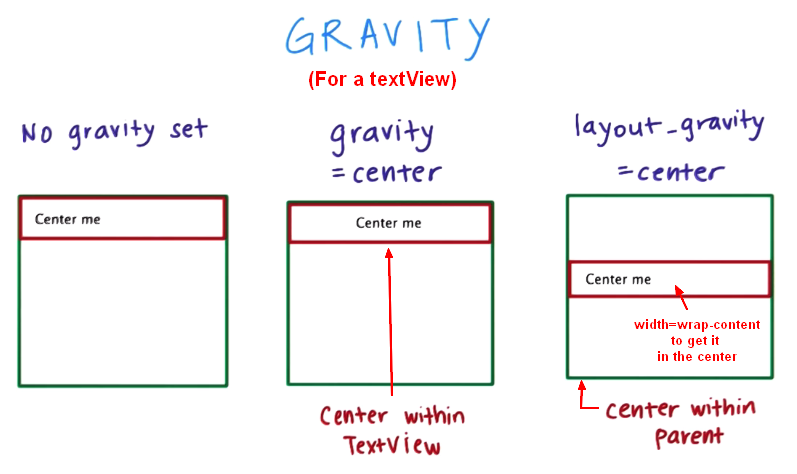
\includegraphics[scale=.35]{gravity.png}
  \caption{Gravity}
  \label{fig:grav}
\end{figure}
\begin{figure}[H]
  \centering
  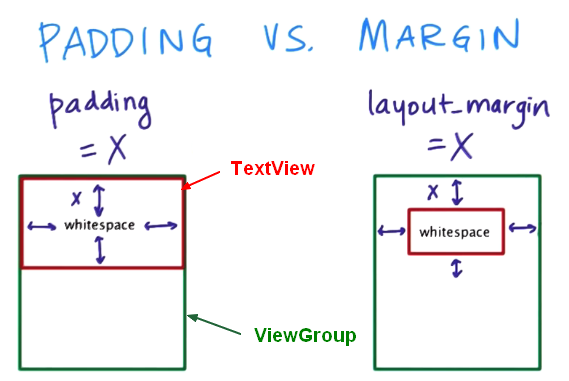
\includegraphics[scale=.35]{padding_margin.png}
  \caption{Padding and margin}
  \label{fig:pam}
\end{figure}



\subsection{Linear layout}
Linear layout places other views either horizontally in a single row or vertically in a single column. The \texttt{orientation} attribute determines its direction. Listing \ref{listing:linlay} shows a linear layout in XML where the orientation is horizontal, so all children will be placed in a single row and they will not wrap if we reach the end of the screen. The gravity centers horizontally and vertically for both orientations. The views are placeholder for any view.
\begin{lstlisting}[style=A_XML, caption={Linear layout declaration}, label = {listing:linlay}]
<LinearLayout xmlns:android="http://schemas.android.com/apk/res/android"
    android:layout_width="match_parent"
    android:layout_height="match_parent"
    android:paddingLeft="16dp"
    android:paddingRight="16dp"
    android:orientation="horizontal"
    android:gravity="center">
    <SomeView> </SomeView>
    <SomeView> </SomeView>
</LinearLayout>
\end{lstlisting}

\subsection{Relative layout}
Relative layouts specify the position of its views relative either it siblings or parent view. Attributes revolve around position relative to others given by id (or their unique parent view). Attributes like \texttt{below} and \texttt{toLeftOf} have view id's as value while alignments relative to parent have boolean values. Listing \ref{listing:rellay} shows example views (using \texttt{SomeView} as a placeholder) positioning in a relative view.
\begin{lstlisting}[style=A_XML, caption={Relative layout declaration}, label = {listing:rellay}]
<RelativeLayout xmlns:android="http://schemas.android.com/apk/res/android"
    android:layout_width="match_parent"
    android:layout_height="match_parent">
    <SomeView
        android:id="@+id/id1"
        android:layout_alignParentTop="true"
        android:layout_marginStart="79dp"
        android:layout_marginTop="111dp" />
    <SomeView
        android:id="@+id/id2"
        android:layout_marginStart="44dp"
        android:layout_marginTop="45dp"
        android:layout_below="@+id/id1"
        android:layout_toEndOf="@+id/id1" />
</RelativeLayout>
\end{lstlisting}

\subsection{Grid layout}
The grid layout places its children with 2d positions in a grid. The column determines where the child lands horizontally and row vertically.
\begin{lstlisting}[style=A_XML, caption={Grid layout declaration}, label = {listing:gridlay}]
<GridLayout xmlns:android="http://schemas.android.com/apk/res/android"
    android:layout_width="match_parent"
    android:layout_height="match_parent">
    <SomeView
        android:layout_column="0"
        android:layout_row="0"/>
    <SomeView
        android:layout_column="1"
        android:layout_row="1"/>
</GridLayout>
\end{lstlisting}

\subsection{Lists view}
List view offer scrollable views of list items. Static lists can be defined with string arrays in the string resource XML file and added with the entries tag as is shown in listings \ref{listing:resarr} and \ref{listing:stalis}.
\begin{lstlisting}[style=A_XML, caption={Resource string array}, label = {listing:resarr}]
<string-array name="arr">
    <item>"item1"</item>
    <item>"item2"</item>
    <item>"item3"</item>
</string-array>
\end{lstlisting}
\begin{lstlisting}[style=A_XML, caption={Static list}, label = {listing:stalis}]
<ListView xmlns:android="http://schemas.android.com/apk/res/android"
    android:layout_width="match_parent"
    android:layout_height="match_parent"
    android:entries="@array/arr"
    android:id="@+id/list_view_example">
</ListView>
\end{lstlisting}

Dynamic lists must be populated in Java with the \texttt{ArrayAdapter} class. Clicking an item in the list does not invoke a \texttt{OnClickEvent} on the item but \texttt{OnItemClickListener}. The populating of a list and a click event is shown in listing \ref{listing:dynlis}. The \texttt{Toast} class is used to create a timed pop up message.

\begin{lstlisting}[style=A_Java, caption={Dynamic list}, label = {listing:dynlis}]
// Set values dynamically
String[] items = new String[]{ "item1", "item2", "item3"};
ArrayAdapter<String> arrayAdapter = new ArrayAdapter<String>(
    this, android.R.layout.simple_list_item_1, items);
ListView lis = (ListView)findViewById (R.id.list_view_example);
lis.setAdapter (aa);
// Set listener when list items are clicked
lis.setOnItemClickListener(new AdapterView.OnItemClickListener() {
    @Override
    public void onItemClick(
        AdapterView<?> parent, View view, int position, long id
    ) {
        String item = (String)parent.getItemAtPosition(position);
        Toast.makeText(MainActivity.this, item, Toast.LENGTH_SHORT).show();
    }
});

\end{lstlisting}

\section{Widgets}
Widgets are the drawable UI components of the android views. We have already seen buttons when we looked at events but there are plenty others available. We will only look at a handful but you are encouraged to look at more. Note that in these examples, we are not storing strings in the resource string file for demonstration purposes but emphasize that they should always be placed there.

\subsection{Text view}
A text view is used to display text. The text can be changed in Java with the \texttt{setText} method and retrieved with the \texttt{getText} method. Note that \texttt{getText} returns a \texttt{CharSequence} rather than a string.
\begin{lstlisting}[style=A_XML, caption={Text view declaration}, label = {listing:dectext}]
<TextView
    android:layout_width="wrap_content"
    android:layout_height="wrap_content"
    android:fontFamily="sans-serif-condensed"
    android:text="My Text View"
    android:textSize="30sp"/> <!-- text should be in res/strings -->
\end{lstlisting}

\subsection{Edit text}
Edit text are used for text input. They have various types that restrict their input, such as numeric, password, email and text. 
\begin{lstlisting}[style=A_XML, caption={Edit text declaration}, label = {listing:edittext}]
<EditText
    android:id="@+id/my_input_form"
    android:layout_margin="15dp"
    android:layout_width="match_parent"
    android:layout_height="wrap_content"
    android:hint="Enter text"
    android:inputType="text" /> <!-- hint should be in res/strings -->
\end{lstlisting}
To access the input, we can use the following code. Watch out for empty inputs or inputs containing white spaces only.
\begin{lstlisting}[style=A_Java]
EditText input = (EditText)findViewById(R.id.my_input_form);
String currentInput = input.getText().toString();
\end{lstlisting}

\subsection{Image view}
Image view can display image resources on screen. Suppose we have an image called image.png that we have placed in the drawable folder, then we can set an image view's src to its name and it will render it on screen.
\begin{lstlisting}[style=A_XML, caption={Image view declaration}, label={listing:img}]
<ImageView
    android:layout_width="wrap_content"
    android:layout_height="250dp"
    android:background="@color/colorAccent"
    android:src="@drawable/image"/>
\end{lstlisting}

\subsection{Radio buttons}
Radio buttons have to be grouped in a container called \texttt{RadioGroup}. If not, choosing one will not cancel another. Toggling a radio button triggers an on click event and all buttons can be set to the same listener.
\begin{lstlisting}[style=A_XML, caption={Radio button declaration}, label={listing:radiodecl}]
<RadioGroup
    android:layout_margin="15dp"
    android:gravity="center"
    android:layout_width="match_parent"
    android:layout_height="wrap_content"
    android:orientation="horizontal">
    <RadioButton
        android:id="@+id/r1"
        android:layout_width="wrap_content"
        android:layout_height="wrap_content"
        android:text="option 1"
        android:onClick="radioClick"/> <!-- text should be in res/strings -->
    <RadioButton
        android:id="@+id/r2"
        android:layout_width="wrap_content"
        android:layout_height="wrap_content"
        android:text="option 2"
        android:onClick="radioClick"/> <!-- text should be in res/strings -->
    <RadioButton
        android:id="@+id/r3"
        android:layout_width="wrap_content"
        android:layout_height="wrap_content"
        android:text="option 3"
        android:onClick="radioClick"/> <!-- text should be in res/strings -->
</RadioGroup>
\end{lstlisting}

In Java, we can find out which button was pushed by getting the id from the \texttt{View} parameter. 

\begin{lstlisting}[style=A_Java, caption={Radio button event}, label={listing:radioev}]
public void radioClick(View view) {
    if (((RadioButton)view).isChecked()) {
        switch (view.getId()) {
            case R.id.r1:
                Toast.makeText(this, "R1", Toast.LENGTH_SHORT).show();
                break;
            case R.id.r2:
                Toast.makeText(this, "R2", Toast.LENGTH_SHORT).show();
                break;
            case R.id.r3:
                Toast.makeText(this, "R3", Toast.LENGTH_SHORT).show();
                break;
        }
    }
}
\end{lstlisting}

\subsection{Spinners}
Spinners are Android's drop down lists. They work similarly to list views and can be populated with string array resources in XML.

\begin{lstlisting}[style=A_XML, caption={Spinner declaration}, label={listing:spinxml}]
<Spinner
    android:id="@+id/my_spinner"
    android:layout_width="match_parent"
    android:layout_height="wrap_content"
    android:entries="@array/arr"/>
\end{lstlisting}

They can also be populated in Java with \texttt{ArrayAdapter} but use a different layout id than list views. The \texttt{onItemSelectedListener} is triggered as soon as an element is selected in the spinner. For spinners with a possible empty choice, the method \texttt{onNothingSelected} is invoked.

\begin{lstlisting}[style=A_Java, caption={Spinner population and event}, label={listing:spinpopev}]
String entries[] = new String[]{"item1", "item2", "item3"};
ArrayAdapter<String> arrayAdapter = new ArrayAdapter<>(
        this, android.R.layout.simple_spinner_item, entries);
Spinner spinner = (Spinner)findViewById(R.id.my_spinner);
spinner.setAdapter(arrayAdapter);
spinner.setOnItemSelectedListener(new AdapterView.OnItemSelectedListener() {
    @Override
    public void onItemSelected(
            AdapterView<?> parent, View view, int position, long id
    ) {
        String msg = parent.getItemAtPosition(position).toString();
        Toast.makeText(MainActivity.this, msg, Toast.LENGTH_SHORT).show();
    }
    @Override
    public void onNothingSelected(AdapterView<?> parent) {
        Toast.makeText(MainActivity.this, "None", Toast.LENGTH_SHORT).show();
    }
});
\end{lstlisting}


\section{Assignment - Simple calculator}
\begin{minipage}{0.45\textwidth}
\begin{figure}[H]
\centering
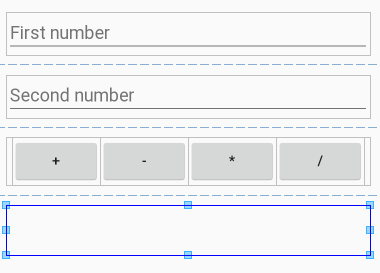
\includegraphics[scale=1]{simple_calculator.png}
\caption{Simple calculator}
\label{fig:simcal}
\end{figure}
\end{minipage}
\hfill
\begin{minipage}{0.475\textwidth}
In this assignment you should design a very simple calculator with two input fields and a result display. It should support addition, subtraction, multiplication and division. The bulk of the Java code is given but you must create the XML layout from scratch. The Java code assumes that an error message is stored in a resource string \texttt{err\_msg}. You must implement the \texttt{onCreate} method in Java as well as the calculations and the resulting display.
\end{minipage}

\begin{lstlisting}[style=A_Java, caption={Assignment template}, label={listing:asigtemp}]
public class MainActivity extends AppCompatActivity {
    private EditText first, second;
    private TextView answer;
    @Override 
    protected void onCreate(Bundle savedInstanceState) {
        // TODO: set fields
    }
    public void calculate(View view) {
        // Check if edit text are empty
        if (first.getText().toString().trim().length() == 0
                    || second.getText().toString().trim().length() == 0) {
            answer.setText(R.string.err_msg);
            return;
        } else {
            try {
                // Convert text fields to integers for arithmetic
                int lhs = Integer.parseInt(first.getText().toString());
                int rhs = Integer.parseInt(second.getText().toString());
                // TODO: calculations based on button pressed
                // TODO: set answer display
            } catch (NumberFormatException ex) {
                answer.setText(R.string.err_msg);
            }
        }
    }
}
\end{lstlisting}
